\documentclass[11pt]{article}
\usepackage[T1]{fontenc}
\usepackage[utf8]{inputenc}
\usepackage{lmodern}
\usepackage[margin=1in]{geometry}
\usepackage{microtype}
\usepackage{amsmath}
\usepackage{booktabs}
\usepackage{tabularx}
\usepackage{graphicx}
\usepackage{caption}
\usepackage{enumitem}
\usepackage[section]{placeins}
\usepackage[numbers,sort&compress]{natbib}
\usepackage{xcolor}
\usepackage[colorlinks=true,linkcolor=black,citecolor=black,urlcolor=blue!50!black,pdftitle={Chronos-2 on Moscow Exchange Equities: Direction, Cross-Sectional Alpha and Risk},pdfauthor={Ilia Mirkis}]{hyperref}

\captionsetup{font=small,labelfont=bf}
\setlist{itemsep=1pt,topsep=3pt}
\newcommand{\repo}{\url{https://github.com/Lutyyyyy/moex-chronos2}}

\title{Chronos-2 on Moscow Exchange Equities:\\Direction, Cross-Sectional Alpha and Risk}
\author{Ilia Mirkis}
\date{September 2026}

\begin{document}
\maketitle

\begin{abstract}
\noindent
We test whether Chronos-2, a pretrained time-series foundation model, improves on standard quantitative tools
for Moscow Exchange (MOEX) equities, in three studies of increasing practical relevance: predicting the sign of
returns, ranking stocks for a long-short portfolio, and forecasting risk (value-at-risk and expected shortfall,
volatility targeting, minimum-variance portfolios and hedging). All model selection used a development period
with every variant logged; the risk study's claims were pre-registered and tested once on a sealed 2025--26
holdout. Directional accuracy is at the no-skill level across resolutions, context lengths, groupings and
sectors. The model's quantile forecasts rank stocks with a real information coefficient (about 0.07), but the
signal is largely explained by known factors and earns no net alpha. For risk, Chronos-2 combined with a
classical model is not meaningfully worse than the best classical model for VaR/ES and hedging
(pre-registered non-inferiority tests, $p < 10^{-5}$) and not significantly better in any use; two development-period advantages shrank or reversed on
the holdout. Across input modes, the forecast target (log realized variance rather than returns) and combination
with classical models mattered more than attention across series or joint multivariate forecasting.
\end{abstract}

\section{Introduction}

Time-series foundation models are pretrained on large collections of series and forecast new ones without
task-specific training. Chronos-2 \citep{ansari2025chronos2} adds group attention, which lets series in a batch
inform each other, and supports multivariate targets and covariates. General forecasting benchmarks rank such
models highly, but financial returns are close to unpredictable by construction, and it is not obvious that
benchmark strength carries over.

This report asks three questions, each motivated by the answer to the previous one:
\begin{enumerate}
  \item \textbf{Direction.} Does Chronos-2 predict the sign of each stock's next return well enough to cover
    trading costs? (Section~\ref{sec:da})
  \item \textbf{Cross-sectional alpha.} Do its quantile forecasts, used as signals, rank stocks into a portfolio
    that earns net alpha beyond standard factors? Is its forecast width a better volatility model?
    (Section~\ref{sec:alpha})
  \item \textbf{Risk.} Does it improve risk decisions (VaR/ES, volatility targeting, minimum-variance portfolios,
    hedging), and do calibration, combination with classical models, multivariate input, covariates or LoRA
    fine-tuning help? (Section~\ref{sec:risk})
\end{enumerate}
Section~\ref{sec:modes} compares the ways the model was run across the three studies, and
Section~\ref{sec:holdout} shows what the single-use holdout changed. Code, configurations, pre-registrations
and all result tables are in the repository (\repo); market data is not redistributed.

\section{Data}\label{sec:data}

Prices come from MOEX AlgoPack through a tested extraction pipeline: 10-minute, hourly and daily bars for a
liquidity-ranked list of 80 shares (selected by current liquidity, so survivorship applies), index and futures series, and
dividend and split information. Several properties of the feed changed the numbers and had to be handled
explicitly:
\begin{itemize}
  \item \textbf{Evening close.} The daily ``close'' is the last print of the evening session (about 23:40) on
    nearly every day since 2021. Studies 2 and 3 rebuild daily prices from the main-session close (the
    18:40 closing-auction bar in the 10-minute data).
  \item \textbf{Dividends.} Adjustments were applied one day late before 2023-07-31, and one announced dividend
    was never paid; both were corrected.
  \item \textbf{Holidays.} Forward-filling a regular calendar turns market holidays into zero returns. Studies 2
    and 3 use an exchange-derived calendar without forward-fill.
  \item \textbf{Futures rolls.} Returns spanning a contract roll are masked.
  \item \textbf{Realized covariance.} Realized covariances from asynchronous 10-minute trades are biased towards
    zero \citep{epps1979comovements}; factor-model arms are calibrated for it.
\end{itemize}
Realized variance (RV) is the sum of squared main-session 10-minute returns plus the squared overnight return.
Studies 2 and 3 use a point-in-time universe (at least 250 observed returns and a liquidity floor): 47--70
names during 2021--24 and 69--78 during the holdout. The periods are: development (dev) 2021--2024 (study 2
used 2024 as a one-shot test first); holdout 2025-01-03 to 2026-09-17 (434 trading days), sealed until the risk
study's final evaluation.

\section{Protocol and statistics}\label{sec:protocol}

\textbf{Protocol.} All selection used dev data. Success criteria were fixed before each test was run, every
variant evaluated was logged in a trial ledger (238 trials in study 2, 265 in study 3), and hypothesis-generating
steps used dates disjoint from their confirmation. Study 3's pre-registration (frozen arms, claims, margins,
power) was committed before any holdout forecast existed, and its evaluator refuses to run without that commit
or a second time. Study 3 separates three kinds of claim: better than weak baselines, better than the best
classical model, and not worse than it (non-inferiority with margins fixed on dev).

\textbf{Statistics.} Forecast losses are compared with Diebold-Mariano tests \citep{diebold1995comparing} with
Newey-West errors \citep{newey1987simple}, and regime differences with Giacomini-White tests
\citep{giacomini2006tests}. VaR/ES pairs are scored with the FZ0 loss \citep{fissler2016higher,patton2019dynamic}
and backtested with Kupiec \citep{kupiec1995techniques}, Christoffersen \citep{christoffersen1998evaluating} and
Acerbi-Sz\'ekely \citep{acerbi2014backtesting} tests. Volatility forecasts use QLIKE \citep{patton2011volatility}.
The economic value of volatility targeting is a performance fee \citep{fleming2001economic} with stationary
bootstrap inference \citep{politis1994stationary}. Alpha is tested with Fama-MacBeth \citep{fama1973risk} and net
spanning regressions, and the deflated Sharpe ratio \citep{bailey2014deflated} is computed at selection.
Multiple testing is controlled with Benjamini-Hochberg \citep{benjamini1995controlling} or Holm
\citep{holm1979simple}.

\section{Study 1: directional accuracy}\label{sec:da}

\textbf{Design.} Zero-shot Chronos-2 forecasts (q10, q50, q90) were scored by directional accuracy (DA), the
share of windows in which the sign of the median forecast matches the realized return, on up to 400
walk-forward windows per configuration, for each (ticker, horizon) cell. With a round-trip cost of about 0.10\%
and a typical move of 1.4\%, a directional bet needs DA $\ge 0.536$ to break even. Seventy configurations
varied resolution (daily, hourly, 10-minute), context length (35, 100, 250 bars), raw versus adjusted prices,
cross-sector versus single-sector baskets, and cross-learning (the model's group attention across the tickers
of a basket) versus independent univariate forecasts. The cross-learning gate compared paired configurations
window by window with McNemar tests \citep{mcnemar1947note}; a lead-lag family screened residualized lagged
cross-correlations on 2020--23 and re-tested the Benjamini-Hochberg shortlist on 2023--24.

\textbf{Results.} Mean DA per run lies between 0.46 and 0.51. Values below 0.5 are expected: a zero realized
return counts as a miss. Zero returns are common in 10-minute bars (6.8\% of bars in the 2023 window, which
puts no-skill DA near 0.47), and they also occur on the holiday rows of this study's forward-filled daily grid. Every pre-registered
gate failed:
\begin{itemize}
  \item \textbf{Cross-learning:} in eight paired runs across three resolutions and three context lengths,
    $|\Delta\text{DA}| \le 0.0018$ and 0 of 64 cells were significant after correction in each
    (Figure~\ref{fig:da}a). Twenty-four single-sector configurations produced one significant cell, with the
    wrong sign.
  \item \textbf{Lead-lag:} 20 residualized pairs were significant on 2020--23; none replicated on 2023--24
    (best corrected $p = 0.70$).
  \item \textbf{The one exception:} one ticker (UNAC) at context 100 reached DA 0.60--0.64 (corrected
    $p = 0.0002$). On a fresh window (2024-11 to 2026-09) it fell to 0.545--0.569 (corrected $p = 0.26$), and the
    earlier result traced to that stock's own momentum after a +157\% price spike, which a naive sign rule
    reproduced. This window overlaps the later risk holdout; it was a directional test of one ticker family.
\end{itemize}
Of 2,920 (ticker, horizon) cells, 74 (2.5\%) exceed the break-even DA, about what sampling noise alone produces
with 400 windows per cell (Figure~\ref{fig:da}b). Ten-minute returns show no autocorrelation for the model to
exploit (mean lag-1 autocorrelation $-0.007$).

\begin{figure}[!htbp]
  \centering
  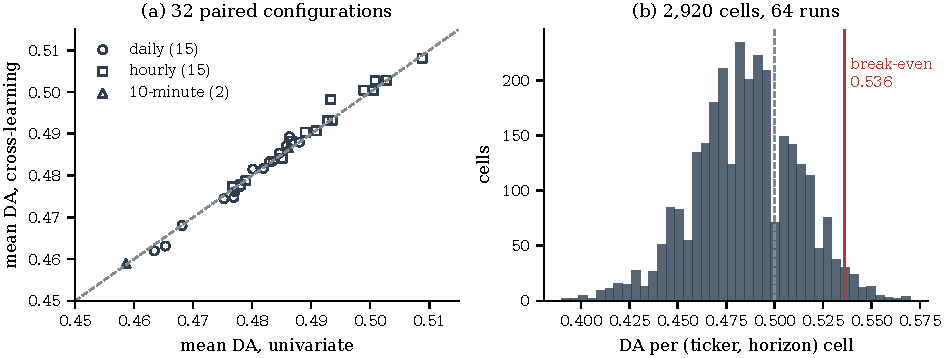
\includegraphics[width=\textwidth]{figures/fig1_directional.pdf}
  \caption{Study 1. (a) Mean primary-horizon DA of cross-learning versus univariate forecasts for 32 paired
  configurations (basket gate and sector baskets); points lie on the diagonal. (b) DA of every (ticker, horizon)
  cell in 64 runs; dashed line 0.5, red line the 0.536 break-even after costs.}
  \label{fig:da}
\end{figure}

\section{Study 2: cross-sectional alpha and volatility}\label{sec:alpha}

\textbf{Design.} A portfolio manager needs relative ranking, not per-stock direction, and can use the forecast
distribution, not only its median. Chronos-2 produced 21-quantile forecasts (context 250, horizon 6) for every
eligible stock on every trading day. The signal was the forecast median over the holding period, scaled by
forecast dispersion. Books were weekly rebalanced, beta-neutral long-short and long-only, with 5~bps one-way
costs plus borrow, and compared against momentum, reversal, low-volatility and AR(1) books built identically. A
one-shot 2024 test was pre-registered first; an improvement wave on 2021--24 followed.

\textbf{Return alpha.} The ranking skill is real but not tradable (Table~\ref{tab:alpha}, Figure~\ref{fig:alpha}a):
\begin{itemize}
  \item Chronos ranks stocks with rank IC 0.07--0.08 ($t$ 6--7) on 2021--24; in 2024 its IC (0.088--0.096) was
    higher than any classic signal's.
  \item A linear ``mimic'' fitted on cheap trailing statistics of each stock reproduces about 45\% of the signal
    and trades better (net Sharpe 2.0 versus 1.2).
  \item The pre-registered 2024 net spanning-alpha leg failed ($t = -0.55$; $-0.97$ after data corrections to dividends and the calendar).
  \item A 20-configuration sweep (cross-learning in four grouping schemes, past covariates, context 64--512,
    residual, weekly and log-price targets) gave a best net spanning $t$ of 0.82. With Brent, USD/RUB and gold
    futures as covariates the model keeps a component the mimic cannot explain (Fama-MacBeth $t = 2.47$, an
    upper bound because the mimic is linear), but that component's own book loses money (net Sharpe $-0.38$),
    its weight in a combination with classic factors is about 0.002, and a Bonferroni bound over 20
    configurations would require $t \approx 3$. Smoothing that signal to cut turnover raised the spanning $t$
    to 1.46, still below 2, and the configuration stays below 2 even at zero cost ($t = 1.71$).
\end{itemize}

\begin{table}[!htbp]
  \centering\small
  \caption{Study 2, 2021--24: Chronos signals versus a linear mimic. FM: Fama-MacBeth $t$ controlling for
  classic factors; spanning: net alpha $t$ against the classic books and the index at 5~bps.}
  \label{tab:alpha}
  \begin{tabular}{lrrrr}
    \toprule
    Signal & IC $t$ & FM $t$ & Spanning $t$ & Net Sharpe \\
    \midrule
    Chronos, univariate & 6.37 & 2.70 & $-0.15$ & 1.17 \\
    Chronos, futures covariates (best of 20) & 6.96 & 4.70 & 0.82 & 1.57 \\
    Linear mimic of the univariate signal & -- & -- & 1.56 & 1.99 \\
    Futures-covariate signal minus extended mimic & -- & 2.47 & $-0.43$ & $-0.38$ \\
    \bottomrule
  \end{tabular}
\end{table}

\textbf{Volatility.} Forecast width from daily returns was no better than EWMA or GARCH(1,1), and its tails were
too narrow in 2024 (6.7\% hits at the 5\% quantile). Run on log realized variance instead, Chronos beats EWMA,
GARCH and HAR-RV \citep{corsi2009simple} (QLIKE 0.50 versus 0.65--0.86), but a pooled log-HAR with a market term
matches it (QLIKE 0.455; Figure~\ref{fig:alpha}b). The edge over the simple models came from working in log space
and pooling across stocks, which classical models can also do. A pre-registered encompassing test found that
Chronos carries information log-HAR lacks (coefficient 0.56, $t = 4.3$), mostly in calm years, but a fixed
combination did not lower QLIKE, and no portfolio use showed an economic gain.

\begin{figure}[!htbp]
  \centering
  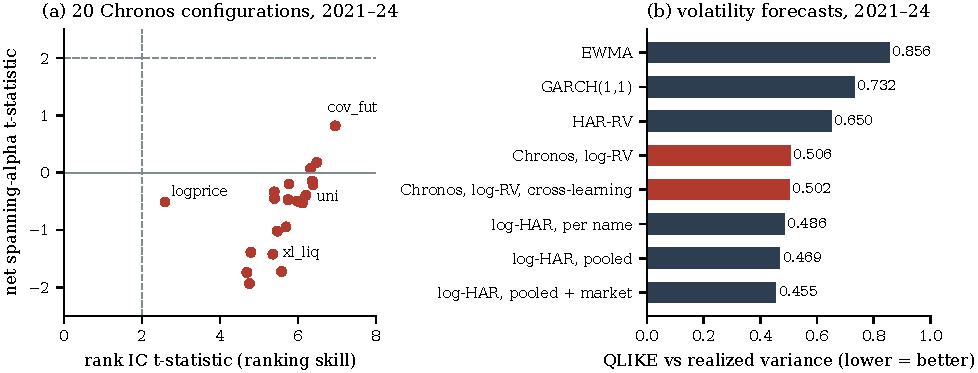
\includegraphics[width=\textwidth]{figures/fig2_alpha.pdf}
  \caption{Study 2, 2021--24. (a) Rank-IC $t$ against net spanning-alpha $t$ for the 20 Chronos configurations:
  every configuration ranks stocks significantly, none earns significant net alpha (dashed lines $t = 2$).
  (b) QLIKE of 5-day variance forecasts against realized variance; Chronos in red.}
  \label{fig:alpha}
\end{figure}

\section{Study 3: risk}\label{sec:risk}

\textbf{Uses.} (U1) one-day 5\% VaR/ES for every stock, scored by FZ0; (U2) volatility targeting an equal-weight
book to 10\%, scored by the performance fee against EWMA; (U3) a long-only minimum-variance portfolio, scored by
realized 5-day variance; (U4) hedging each stock with the IMOEX future, scored by hedged 5-day variance.

\textbf{Arms.} Zero-shot Chronos on returns, on log RV and on both jointly; calibrated and filtered-historical-
simulation (FHS) \citep{baroneadesi1999var} versions; fixed, fitted and regime-dependent mixtures with the best
classical model; a one-factor covariance model with Chronos market and residual variances; market and macro
covariates; and LoRA \citep{hu2022lora} fine-tuning (rank 8) with yearly refits trained only on data before each
year. Classical rivals: RiskMetrics/EWMA \citep{riskmetrics1996}, GARCH and GARCH-t, historical simulation and FHS,
HAR and log-HAR variants, and a rolling OLS beta for hedging. One arm per use was frozen on dev; a fine-tuned arm
replaced it only if it had lower loss on 2022--24, which happened for U1 and U3. The frozen arms are: U1, a
50/50 mixture of fine-tuned multivariate Chronos return quantiles and FHS log-HAR; U2, the one-factor model;
U3, a 50/50 mixture of fine-tuned Chronos variance and pooled log-HAR; U4, a calibrated mixture of zero-shot
Chronos log-RV and pooled log-HAR.

\textbf{Claims.} Family A (``better than''): beat both reference arms (L1), then the best classical arm (L2), plus
a calm-day VaR claim (R), Holm-corrected across uses. Family B (``not worse''): non-inferiority against the best
classical arm with margins fixed on dev (U1: 0.063 FZ0, half of the best model's dev gain over RiskMetrics; U4:
+0.5 percentage points of annual hedged volatility). U2 and U3 had no non-inferiority test because their holdout
standard errors were too large. The holdout was evaluated once, on 395--433 forecast dates per use.

\textbf{Results.} Chronos-2 reaches parity with the best classical risk models but no demonstrated advantage
(Tables~\ref{tab:claims} and~\ref{tab:uses}, Figure~\ref{fig:risk}). Both non-inferiority claims pass by a wide
margin, and Chronos has the best point estimate for VaR/ES and hedging, but no ``better than'' claim survives the
correction. EWMA remains best for minimum-variance portfolios, and GARCH and a log-HAR model of portfolio
variance beat the Chronos volatility-targeting book. The Chronos VaR arm has a 4.77\% hit rate (Kupiec
$p = 0.056$), against 5.35\% for RiskMetrics and 5.65\% for GARCH-t, whose coverage is rejected.

\begin{table}[!htbp]
  \centering\small
  \caption{Study 3: confirmatory claims on the holdout (2025-01 to 2026-09), one-sided tests.}
  \label{tab:claims}
  \begin{tabularx}{\textwidth}{Xlll}
    \toprule
    Claim & Statistic & Raw $p$ & Holm \\
    \midrule
    Not worse, VaR/ES (margin 0.063 FZ0) & upper 95\% bound $+0.003$ & $8\times10^{-17}$ & pass \\
    Not worse, hedging (margin $+0.5$ pp vol) & bound $1.3$ vs margin $6.6$ ($\times10^{-5}$) & $8\times10^{-6}$ & pass \\
    L1 VaR/ES: beats RiskMetrics and GARCH-t & $t = -1.87$ / $-2.37$ & 0.031 & fail \\
    R: VaR/ES beats FHS log-HAR, calm days & $t = -1.31$ (381 days) & 0.095 & fail \\
    L1 vol targeting / min-variance / hedging & Table~\ref{tab:uses} & 0.71 / 0.92 / 0.48 & fail \\
  \end{tabularx}
\end{table}

\begin{table}[!htbp]
  \centering\small
  \caption{Study 3: holdout losses per use. Lower is better except for the fee, which is relative to each
  comparison arm, so the Chronos column has no standalone value.}
  \label{tab:uses}
  \begin{tabularx}{\textwidth}{llXX}
    \toprule
    Use & Chronos & Best classical & Baselines \\
    \midrule
    VaR/ES, FZ0 & $\mathbf{-3.082}$ & FHS log-HAR $-3.070$ & GARCH-t $-3.043$; RiskMetrics $-3.032$ \\
    Vol targeting, fee of Chronos (bps/yr) & -- & $-128$ vs log-HAR on portfolio RV & $+243$ vs EWMA; $-72$ vs GARCH \\
    Min-variance, annual vol & 17.74\% & \textbf{EWMA 16.85\%} & GARCH 18.29\% \\
    Hedging, hedged annual vol & \textbf{31.13\%} & OLS beta 31.30\% & EWMA 31.14\%; GARCH 31.62\% \\
    \bottomrule
  \end{tabularx}
\end{table}

\begin{figure}[!htbp]
  \centering
  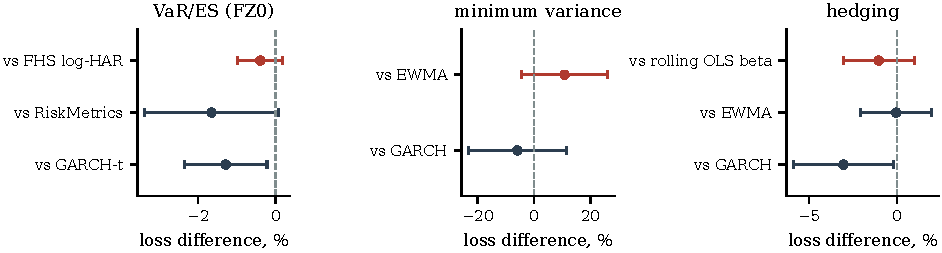
\includegraphics[width=\textwidth]{figures/fig3_holdout_effects.pdf}
  \caption{Study 3, holdout. Loss difference of the frozen Chronos arm against each classical arm, in \% of the
  reference arm's loss, with 95\% Newey-West intervals (left of zero: Chronos better). Red: against the best
  classical model.}
  \label{fig:risk}
\end{figure}

\textbf{What helped on dev.} Mixing Chronos 50/50 with a classical model beat Chronos alone in every use;
three of the four frozen arms are such mixtures. Covariates, the Chronos model of the correlation side and
fine-tuning on log-RV alone showed no measurable gain. Only weak baselines (RiskMetrics, GARCH-t, GARCH) were
beaten significantly on dev.

\section{Which Chronos-2 modes worked}\label{sec:modes}

Across the studies the model was run in most of its available modes. Table~\ref{tab:modes} compares each mode
with the plain univariate call; study 1's ``multivariate'' grouping is the cross-learning flag, and
\emph{multivariate} here means return and log RV of the same stock forecast jointly. The study 3 $t$-statistics
are dev Diebold-Mariano tests on arms already in the ledger, computed after the holdout and not corrected for
multiplicity.

\begin{table}[!htbp]
  \centering\small
  \caption{Input modes against the univariate call (dev unless noted). $t$: Diebold-Mariano $t$ of the loss
  difference, negative favours the mode.}
  \label{tab:modes}
  \begin{tabularx}{\textwidth}{lX}
    \toprule
    Mode & Effect \\
    \midrule
    Cross-learning across tickers & Direction: no effect ($|\Delta\text{DA}| \le 0.0018$). Ranking: weaker (IC $t$
      5.47 vs 6.37). Volatility from return forecasts: better (scaled QLIKE $t = -3.77$); on log RV none (QLIKE
      0.501 vs 0.504). VaR from return quantiles: worse ($t = +1.84$). \\
    Multivariate [return, log RV] & VaR quantiles better ($t = -3.35$ against the same cross-learning call
      without log RV, $-1.62$ against univariate); variance forecasts worse than log RV alone (QLIKE 0.598 vs
      0.554, $t = +1.50$; minimum-variance $t = +1.83$). \\
    Target other than returns & Log RV: the largest single effect (QLIKE 0.554 vs 0.890, $t = 3.05$). Log price:
      ranking destroyed (IC $t$ 2.59 vs 6.37). \\
    Past covariates & Ranking: largest gain (Fama-MacBeth $t$ 4.09 beyond univariate) but net spanning $t$ 0.82.
      Risk: no measurable gain. \\
    Context length & Direction: 35, 100 and 250 all null. Ranking: 250 best (IC $t$ 6.37 vs 4.8--5.4). \\
    LoRA fine-tuning & Multivariate: better than zero-shot in 21 of 22 arms on 2022--24; on the holdout worse for
      VaR ($t = +1.07$), insignificant for minimum variance ($t = -0.57$). Log RV only: never significant. \\
    \bottomrule
  \end{tabularx}
\end{table}

Attention across tickers helped only the volatility read from return quantiles. Joint forecasting helped the
return side and hurt the variance side, and only one of these differences clears $|t| = 2$. The choices that
mattered were the target and the use of the output: forecasting log RV rather than returns, converting its
variance into VaR by FHS rather than reading return quantiles (FZ0 $-3.055$ vs $-2.970$, $t = -1.59$), and
combining with a classical model. A multivariate variant on 5-day blocks tied univariate log RV on variance but
produced failed hedges in the 2022 stress (stress-day hedged volatility 381\% against 40\%). No mode changed a
verdict.

\section{What the holdout changed}\label{sec:holdout}

Figure~\ref{fig:holdout} shows the same comparisons computed by the same code on dev and on the holdout. The
calm-day VaR advantage, the strongest dev result ($t = -4.0$, expected holdout $t \approx -2.7$ at the dev effect
size), fell to $t = -1.3$, consistent with a winner's curse from selecting the best of 265 variants. The
fine-tuning gain over zero-shot reversed sign for VaR and weakened for minimum variance, and the calm-day pattern
reversed for minimum variance. Other comparisons moved in Chronos's favour (VaR against FHS log-HAR, hedging
against OLS beta). Movements of this size in both directions are what the short holdout allows, which is why
non-inferiority was pre-registered alongside the superiority claims.

\begin{figure}[!htbp]
  \centering
  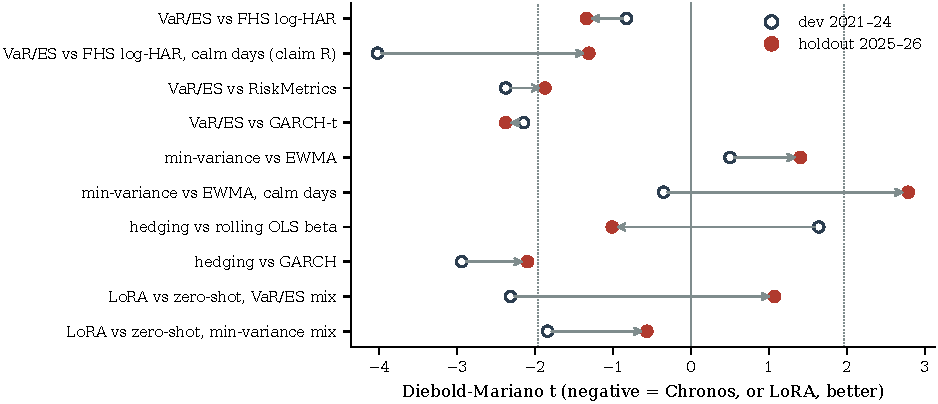
\includegraphics[width=\textwidth]{figures/fig4_dev_vs_holdout.pdf}
  \caption{Diebold-Mariano $t$-statistics of the frozen comparisons on dev (open) and holdout (filled), computed
  by the holdout evaluation code in both periods (dev values from its dry run on 2021--24); dotted lines
  $\pm 1.96$.}
  \label{fig:holdout}
\end{figure}

\section{Discussion and limitations}\label{sec:discussion}

Chronos-2 has no directional edge and no tradable alpha on MOEX equities. For risk it reaches, but does not
exceed, the best classical models, at a higher computational cost: a transformer forward pass per forecast date
and a GPU for fine-tuning, against closed-form or small-regression classical models. Where it was competitive,
the gains came from choices classical models can also make (log space, pooling across stocks, combination).

The safeguards changed the conclusions several times: a lead-lag shortlist dominated by a market factor
(19 of 20 pairs shared one lag), the UNAC result, an evaluation universe that silently dropped the 2022 crash
months until a dry run of the holdout code exposed it, a median-based calibration that left volatility-targeted
books at 18--20\% instead of 10\%, and the two dev advantages above.

\textbf{Limitations.} One market and one period (2020--2026), with a universe selected by current liquidity. A
null at these sample sizes does not rule out a narrow, regime-specific edge. The holdout is short, so the
superiority tests had low power for most uses. Whether MOEX series were in Chronos-2's pretraining data is
unknown. Ticker grouping for the joint multivariate mode was not varied; a real test would need a grouping
chosen in advance and fresh data.

{\small\setlength{\bibsep}{1pt}
\bibliographystyle{plainnat}
\bibliography{refs}}

\end{document}
